\documentclass[a4paper,11pt,UTF8]{article}
\usepackage{ctex}
\usepackage{amsmath,amsthm,amssymb,amsfonts}
\usepackage{amsmath}
\usepackage[a4paper]{geometry}
\usepackage{graphicx}
\usepackage{microtype}
\usepackage{siunitx}
\usepackage{booktabs}
\usepackage[colorlinks=false, pdfborder={0 0 0}]{hyperref}
\usepackage{cleveref}
\usepackage{esint} 
\usepackage{graphicx}
\usepackage{ragged2e}
\usepackage{pifont}
\usepackage{extarrows}
\usepackage{mathptmx}
\usepackage{float}
\usepackage{caption}
\captionsetup[figure]{name={Figure}}
%opening
\title{Microelectronics Circuit Analysis and Design Homework(1st)}
\author{Yuejin Xie \quad U202210333}
\date{Sept 1st, 2023 }
\begin{document}
\maketitle
9.6 Assume the op-amps in Figure P9.6 are ideal. Find the voltage gain
$A_v = v_O /v_I$ and the input resistance $R_i$ of each circuit.
\begin{figure}[H] %H为当前位置,!htb为忽略美学标准,htbp为浮动图形
	\centering %图片居中
	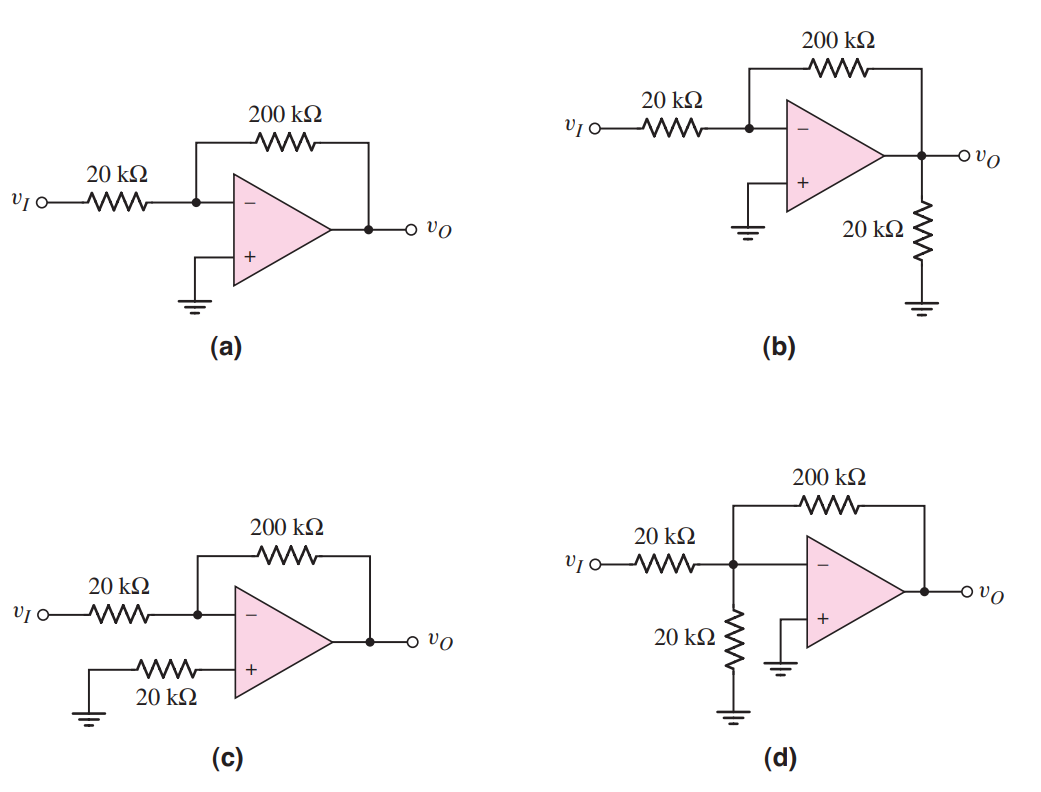
\includegraphics[width=0.7\textwidth]{MD9.6.png} %插入图片,[]中设置图片大小,{}中是图片文件名
	\caption{Problem 9.6}
\end{figure}
\noindent Solution:\\
(a)Actually,$(v_2-v_1)\rightarrow0,i_+,i_-\rightarrow0$, and we have these equations as follow:\\
$\begin{cases}\displaystyle
	\frac{v_I-v_-}{20k\Omega}=\frac{v_--v_O}{200k\Omega}\\
	v_+=0
\end{cases}\Rightarrow \displaystyle\frac{v_O}{v_I}=-10$\\
The input resistance $\displaystyle R_i=\frac{v_I}{\displaystyle\frac{v_I-v_-}{20k\Omega}}=20k\Omega$\\
(b)(c)(d) In fact the new resistances of $20k\Omega$ in Figure (a)(b)(c) don't make differences to their circuits.\\
So the answers do not change: $\displaystyle\frac{v_O}{v_I}=-10, R_i=20k\Omega$\\
9.14 (a) The input to the circuit shown in Figure P9.14 is $v_I = -0.20$ V. (i) What
is $v_O $? (ii) Determine $i_2, i_O$ , and $i_L$ . (b) Repeat part (a) for $v_I = +0.05$ V.
(c) Repeat part (a) for $v_I$ = $8 sin\omega t$ mV.
\begin{figure}[H] %H为当前位置,!htb为忽略美学标准,htbp为浮动图形
	\centering %图片居中
	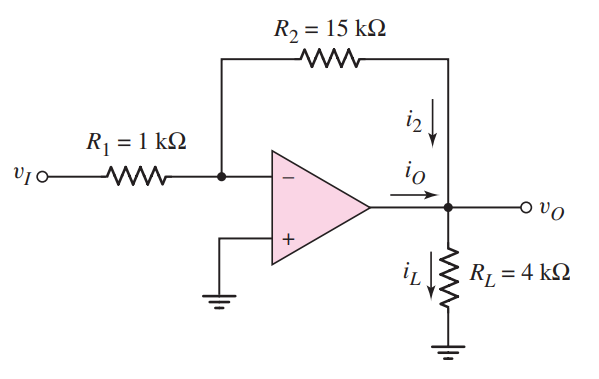
\includegraphics[width=0.5\textwidth]{MD9.14.png} %插入图片,[]中设置图片大小,{}中是图片文件名
	\caption{Problem 9.14}
\end{figure}
\noindent Solution:\\
We provide a general solution in most instances first.\\
Because of "virtual short" , "virtual open" and KCL , we have euqations as follow:\\
$\begin{cases}\displaystyle
	\frac{v_I-v_-}{R_1}=\frac{v_--v_O}{R_2}=i_2\\
	v_+=v_-=0\\
	i_O+i_2=i_L\\
	i_L=\displaystyle\frac{v_O}{R_L}
\end{cases}\Rightarrow 
\begin{cases}\displaystyle
	v_O=-\frac{R_2}{R_1}v_I\\
	i_2=\displaystyle\frac{v_I}{R_1}\\
	i_O=\displaystyle\frac{v_O}{R_L}-\frac{v_I}{R_1}\\
	i_L=\displaystyle\frac{v_O}{R_L}
\end{cases}$\\
(a)$v_O=3V,i_2=-0.2mA,i_O=0.95mA,i_L=0.75mA$\\
(b)$v_O=-0.75V,i_2=0.05mA,i_O=-0.2375mA,i_L=-0.1875mA$\\
(c)$v_O=-120\sin\omega t V,i_2=8\sin\omega t mA,i_O=-38\sin\omega t mA,i_L=-30\sin\omega t mA$\\
9.37 A summing amplifier can be used as a digital-to-analog converter (DAC).
An example of a 4-bit DAC is shown in Figure P9.37. When switch $S_3$ is
connected to the -5 V supply, the most significant bit is $a_3 = 1$; when $S_3$ is
connected to ground, the most significant bit is $a_3 = 0$. The same condition
applies to the other switches $S_2, S_1$, and $S_o$, corresponding to bits $a_2, a_1,$ and
$a_o$, where $a_o$ is the least significant bit. (a) Show that the output voltage is
given by
$$
v_O=\frac{R_F}{10}\left[\frac{a_3}{2}+\frac{a_2}{4}+\frac{a_1}{8}+\frac{a_o}{16}\right](5)
$$
(5)
where $R_F$ is in $k\Omega$. (b) Find the value of $R_F$ such that $v_O = 2.5 V$ when the
digital input is $a_3a_2a_1a_o = 1000$. (c) Using the results of part (b), find $ v_o$
for: (i) $a_3a_2a_1a_o = 0001$, and (ii) $a_3a_2a_1a_o = $.
\begin{figure}[H] %H为当前位置,!htb为忽略美学标准,htbp为浮动图形
	\centering %图片居中
	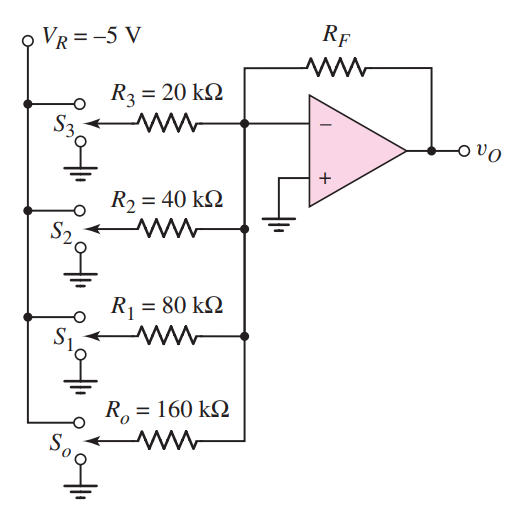
\includegraphics[width=0.4\textwidth]{MD9.37.png} %插入图片,[]中设置图片大小,{}中是图片文件名
	\caption{Problem 9.37}
\end{figure}
\noindent Solution:\\
(a)Because of "virtual short" , "virtual open" , we have euqations as follow:\\
$\begin{cases}\displaystyle
	a_o\frac{v_R-v_-}{R_o}+a_1\frac{v_R-v_-}{R_1}+a_2\frac{v_R-v_-}{R_2}+a_3\frac{v_R-v_-}{R_3}=\frac{v_--v_O}{R_F}\\
	v_+=v_-=0
\end{cases}\\\Rightarrow \displaystyle v_O=\frac{R_F}{2}\left[\frac{a_3}{2}+\frac{a_2}{4}+\frac{a_1}{8}+\frac{a_o}{16}\right]$(Maybe there is a problem with this question?)\\
(b)substitute$v_O = 2.5 V$, $a_3a_2a_1a_o = 1000$ into the (5) $\Rightarrow R_F=10k\Omega$\\
(c)Now $R_F=10k\Omega$\\
so (i) substitute $a_3a_2a_1a_o = 0001$ into the (5) $\Rightarrow v_O= 0.3125V$\\
so (ii) substitute $a_3a_2a_1a_o = 1111$ into the (5) $\Rightarrow v_O=4.6875V$\\
\end{document}